%% 高级图论课程论文
%% 基于《计算机学报》单栏 CjC 模板（Overleaf: latextemplet-CjC-xelatex）
%% 编译方式：XeLaTeX；请将本文件与 figures/、ref.bib 放入模板工程后编译
\documentclass[10.5pt,compsoc,UTF8]{CjC}
\usepackage{CTEX}
\usepackage{graphicx}
\usepackage{footmisc}
\usepackage{subfigure}
\usepackage{url}
\usepackage{multirow}
\usepackage{multicol}
\usepackage[noadjust]{cite}
\usepackage{amsmath,amsthm}
\usepackage{amssymb,amsfonts}
\usepackage{booktabs}
\usepackage{color}
\usepackage{ccaption}
\usepackage{float}
\usepackage{fancyhdr}
\usepackage{caption}
\usepackage{xcolor,stfloats}
\usepackage{comment}
\setcounter{page}{1}
\graphicspath{{figures/}}
\usepackage{cuted}
\usepackage{captionhack}
\usepackage{epstopdf}
\usepackage{gbt7714}

%===============================%
\headevenname{\mbox{\quad} \hfill  \mbox{\zihao{-5}{ \hfill 《高级图论》课程论文  } \hspace {50mm} \mbox{2026 年 7 月}}}%
\headoddname{杜昊存 \hfill 基于图结构的任意字段集合敏感度评估与高阶协同泄露推断}%

\renewcommand{\thefootnote}{\fnsymbol{footnote}}
\setcounter{footnote}{0}
\renewcommand\footnotelayout{\zihao{5-}}

\newtheoremstyle{mystyle}{0pt}{0pt}{\normalfont}{1em}{\bf}{}{1em}{}
\theoremstyle{mystyle}
\newtheorem{definition}{定义}
\newtheorem{proposition}{命题}
\renewcommand\figurename{图~}
\renewcommand{\thesubfigure}{(\alph{subfigure})}
\newcommand{\upcite}[1]{\textsuperscript{\cite{#1}}}
\renewcommand{\labelenumi}{(\arabic{enumi})}
\newcommand{\tabincell}[2]{\begin{tabular}{@{}#1@{}}#2\end{tabular}}
\renewcommand{\bibsection}{}
\makeatletter
\renewcommand{\@biblabel}[1]{[#1]\hfill}
\makeatother
\setlength\parindent{2em}

\begin{document}

\hyphenpenalty=50000
\thispagestyle{plain}%
\thispagestyle{empty}%
\pagestyle{CjCheadings}

\vspace {-13mm}
\onecolumn
\zihao{5-}\noindent 杜昊存 \hfill 《高级图论》课程论文\hfill 2026 年 7 月\\
\noindent\rule[0.25\baselineskip]{\textwidth}{1pt}

{
\centering
\vspace {11mm}
{\zihao{2} \heiti 基于图结构的电网数据任意字段集合敏感度评估\\与高阶协同泄露推断}

\vskip 5mm

{\zihao{4}\fangsong 杜昊存}

\vspace {5mm}

\zihao{5}{(西安交通大学\quad 西安\quad 710049)}
}

\vskip 5mm

\zihao{5}{
\setlength{\baselineskip}{16pt}\selectfont{
\noindent {\heiti 摘\quad 要\quad }
电网运行数据在共享前通常仅删除机密字段，然而剩余字段间的物理与统计耦合使攻击者仍可训练推断模型间接恢复机密量，即数据推断泄露。已有工作（如 IGNN）给每个字段输出单点敏感度分数，本文通过实测指出该刻画的不适定性：泄露本质上是可见字段\textbf{集合}上的集合函数，存在“单看安全、合体泄露”的协同效应——在 PJM 电网 44 字段真实数据上，风电出力与风电占比两字段单独推断总发电量的 $R^2$ 仅为 0.064 与 0.162，合并后升至 0.928，协同增量达 0.765。为此，本文将敏感度升维为任意字段集合的集合函数 $v_c(S)$，并给出一套以图结构为骨架的评估框架：(1) 由字段间推断关系构建相关图，训练图结构专用推断模型作为攻击上限的经验刻画，其在 5 字段以上的随机集合上平均 $R^2$ 高于 MLP 基线（5--8 字段段提升 0.023），且逐集合胜率随集合规模从 20\%单调上升至 90\%；(2) 训练子集条件图 oracle 以一次前向近似任意集合的重训敏感度，经 $K{=}200$ 步微调后对重训真值的逐机密字段 MAE 由 0.136 降至 0.078，集合排序 Spearman 相关达 0.97 以上；(3) 提出“估计器全扫描 + 重训认证”两层协议，在 $\binom{44}{3}=13244$ 个三元组空间中定位真不可约三阶协同：估计与认证排序的 Spearman 相关为 0.795 且估计系统性保守，认证发现最强三阶协同“燃气出力 + 燃气占比 + 负荷预测 $\to$ 净交换功率”达 0.455，而随机对照组 2400 条认证记录中仅 19 条超过显著阈值，证明高阶协同泄露是稀疏结构。实验同时表明，基于置零的敏感度口径较重训真值系统性低估协同 3.4 倍、排序相关仅 0.351，说明忠实的集合敏感度评估必须以重训为真值。
\par}}
\vspace {5mm}

\zihao{5}{\noindent
{\heiti 关键词 \quad }图神经网络；数据推断泄露；集合函数；协同效应；数据脱敏；电力信息物理系统
}

\vskip 7mm

\begin{center}
\zihao{3}{ \heiti Graph-Structured Sensitivity Assessment of Arbitrary Field Subsets and Higher-Order Synergistic Leakage Inference for Power Grid Data}\\
\vspace {5mm}
\zihao{5}{ DU Hao-Cun}\\
\vspace {2mm}
\zihao{5-}{{(Xi'an Jiaotong University, Xi'an 710049, China)}}
\end{center}

\zihao{5}{
\setlength{\baselineskip}{18pt}\selectfont{
{\bf Abstract}\quad
Operational power grid data are usually desensitized by simply removing confidential fields before sharing. However, the physical and statistical couplings among the remaining fields still allow an attacker to train inference models and indirectly recover confidential quantities, a threat known as data inference leakage. Existing approaches such as IGNN assign a single sensitivity score to each field. This paper empirically shows that such a pointwise characterization is ill-posed: leakage is essentially a set function over subsets of visible fields, exhibiting strong synergy where individually harmless fields become highly revealing when combined. On real PJM data with 44 fields, wind generation (MW) and wind share individually infer total generation with $R^2$ of only 0.064 and 0.162, yet jointly reach 0.928, a synergy gain of 0.765. We therefore lift sensitivity to a set function $v_c(S)$ over arbitrary field subsets and propose a graph-structured assessment framework. First, an inference-relation graph over fields is constructed, and a graph-structured dedicated attacker is trained as an empirical upper bound of leakage; it outperforms an MLP baseline on random subsets with five or more fields (up to +0.023 mean $R^2$ on the 5--8 band), with its per-subset win rate increasing monotonically from 20\% to 90\% as subset size grows. Second, a subset-conditional graph oracle trained with random subset dropout approximates the retraining-based sensitivity of any subset in a single forward pass; after $K{=}200$ fine-tuning steps its per-confidential-field MAE against retraining ground truth drops from 0.136 to 0.078, while the Spearman correlation of subset ranking exceeds 0.97. Third, a two-tier ``scan-then-certify'' protocol scans all $\binom{44}{3}=13244$ field triples with the fine-tuned oracle and certifies top candidates by full retraining. The estimated and certified rankings correlate at Spearman 0.795 with the estimator being systematically conservative. Certification reveals the strongest irreducible third-order synergy, ``gas MW + gas share + load forecast $\to$ net interchange'', reaching 0.455, whereas only 19 of 2400 certified records in a random control group exceed the significance threshold, demonstrating that higher-order synergistic leakage is a sparse structure. Experiments further show that zeroing-based sensitivity underestimates synergy by 3.4 times with a rank correlation of merely 0.351 against retraining truth, indicating that faithful subset sensitivity assessment must be grounded in retraining.
\par}}
\vspace {5mm}

{{\bf Keywords}\quad graph neural network; data inference leakage; set function; synergy; data desensitization; cyber-physical power system\par}

\zihao{5}
\vskip 10mm

%%%%%%%%%%%%%%%%%%%%%%%%%%%%%%%%%%%%%%%%%%
\section{\heiti 引言}

现代电力信息物理系统的调度、市场与规划环节依赖细粒度运行数据的交换与共享。共享前的脱敏处理通常只是删除机密字段本身，但保留字段之间存在由物理定律（潮流方程、功率平衡）与统计规律（负荷周期性、气象相关性）决定的强耦合，攻击者可以利用公开字段训练推断模型，间接恢复被删除的机密量，这一威胁被称为数据推断泄露（Data Inference Leakage）\upcite{hu2026ignn}。

针对该威胁，Hu 等人提出的 IGNN\upcite{hu2026ignn} 构建字段间推断关系图并用图神经网络为每个字段输出敏感度分数，是该问题的领域锚点工作。然而，以“单字段分数”刻画泄露存在一个根本性缺陷：\textbf{泄露是可见字段集合上的集合函数，而非单字段的属性}。本文在 PJM 电网真实数据上观测到大量“单看安全、合体泄露”的实例：风电出力（MW）与风电占比两个字段单独推断总发电量的测试 $R^2$ 分别仅为 0.064 与 0.162，接近无泄露；而两者合并后 $R^2$ 升至 0.928——因为总发电量在物理上恰等于出力除以占比。任何单字段评分体系都无法表达这类协同泄露，将敏感度评估建立在单点分数之上是不适定的。

将敏感度升维为集合函数后立刻面临组合爆炸：$n=44$ 个字段的可见集合有 $2^{44}$ 个，逐一重训攻击者不可行。本文以图结构为骨架给出一套可扩展的评估框架，主要贡献如下：

(1) \textbf{问题形式化}。将字段敏感度定义为任意可见集合 $S$ 的集合函数 $v_c(S)$（以重训攻击者的测试 $R^2$ 为语义），并在其上定义二阶与三阶不可约协同，将泄露结构组织为字段集上的协同图与协同超图。

(2) \textbf{图结构专用推断模型}。以字段为节点、推断相关性为边构建相关图，训练可见性感知的图卷积攻击者。在 50 个宽尺寸随机集合上，其平均 $R^2$ 较 MLP 基线整体高 0.007，其中 5--8 字段段高 0.023，且逐集合胜率随集合规模由 20\%单调上升至 90\%，表明图结构先验对中大规模集合的推断具有系统性优势，且两种结构存在互补性（取逐机密字段较优者可再提升 0.005--0.017）。

(3) \textbf{子集条件图 oracle}。以随机子集失活方式联合训练一个对任意掩码集合条件化的图估计器，一次前向即可近似 $v_c(S)$；配合每集合约 3 秒的 $K{=}200$ 步微调，对重训真值的逐机密字段 MAE 由 0.136 降至 0.078，集合排序 Spearman 相关达 0.97--0.99，将单次评估成本从一次完整重训降至秒级。

(4) \textbf{扫描—认证协议与三阶协同发现}。用微调 oracle 全扫描 $\binom{44}{3}=13244$ 个三元组，对 top 候选与随机对照共约 400 个三元组做重训认证。估计与认证排序 Spearman 相关 0.795 且估计保守（不漏强项）；认证发现最强真不可约三阶协同“燃气出力 + 燃气占比 + 负荷预测 $\to$ 净交换功率”达 0.455，其物理机制为“净交换 = 发电 $-$ 负荷”的三字段缺一不可；随机对照组 2400 条认证记录中仅 19 条超过显著阈值，证明高阶协同是稀疏结构，扫描—认证协议因此可以在指数空间中可靠定位少数“针”。

此外，实验对基于置零（将不可见字段置零后测残余精度）的敏感度口径给出了定量否定：置零协同与重训真值的 Spearman 相关仅 0.351，均值低估 3.4 倍，说明忠实的集合敏感度评估必须以重训为真值。

\section{\heiti 相关工作}

\textbf{数据敏感度评估与推断泄露}。IGNN\upcite{hu2026ignn} 融合模型驱动与数据驱动相关性构建推断关系图，以图神经网络输出字段级敏感度。本文与其在“用图组织字段间推断关系”上一脉相承，但将单字段分数升维为任意集合的集合函数，并指出其置零式评估口径会系统性低估协同泄露。

\textbf{特征归因与交互指标}。SHAP\upcite{lundberg2017shap} 及其摊销加速 FastSHAP\upcite{jethani2022fastshap}、ViT-Shapley\upcite{covert2023vitshapley} 研究固定模型下特征子集的边际贡献，Grabisch 等人\upcite{grabisch1999interaction} 给出合作博弈中交互指标的公理化。与之不同，本文的 $v_c(S)$ 对每个集合允许攻击者\textbf{重新训练至最优}（上确界语义），刻画的是攻击者能力上限而非某个固定模型的行为；Datamodels\upcite{ilyas2022datamodels} 在训练子集维度做了类似的“子集 $\to$ 性能”函数拟合，可视为训练侧的平行工作。

\textbf{任意条件建模与缺失特征学习}。VAEAC\upcite{ivanov2019vaeac} 与 ACFlow\upcite{li2020acflow} 学习对任意观测子集条件化的生成模型，GRAPE\upcite{you2020grape} 将缺失特征学习建模为二部图上的表示学习。本文的子集条件 oracle 借鉴了任意条件化思想，但学习目标不是数据分布本身，而是“集合 $\to$ 重训攻击精度”这一集合函数。

\textbf{图神经网络}。GCN\upcite{kipf2017gcn} 与 GAT\upcite{velickovic2018gat} 是本文图结构模型的基础组件；Battaglia 等人\upcite{battaglia2018relational} 系统论述了关系归纳偏置的适用条件，Grinsztajn 等人\upcite{grinsztajn2022tabular} 则指出深度结构先验在表格数据上并非总是有效，这两点共同构成本文第 6 节讨论图结构适用边界的理论背景。

\section{\heiti 问题形式化：作为集合函数的泄露}

\subsection{集合敏感度}

设数据表包含字段集 $F=\{f_1,\dots,f_n\}$（本文 $n=44$），其中机密字段集 $C\subset F$（$|C|=12$）。攻击者可见某个字段集合 $S\subseteq F$，目标是恢复机密字段 $c\in C\setminus S$。

\textbf{定义 1（集合敏感度）}.\quad 给定机密字段 $c$ 与可见集合 $S$，集合敏感度定义为
\begin{equation}
v_c(S)=\max\Bigl(0,\ \sup_{g\in\mathcal{G}}\ R^2_{\mathrm{test}}\bigl(g(X_S)\to x_c\bigr)\Bigr),
\label{eq:vcs}
\end{equation}
其中 $\mathcal{G}$ 为攻击者模型族，$X_S$ 为仅保留 $S$ 中字段的数据。上确界语义强调 $v_c(S)$ 刻画的是\textbf{攻击者最优响应}：对每个 $S$ 攻击者可从头重训至最优，而非在某个固定模型上做特征扰动。实践中以“在多种结构（MLP 与图结构）上重训并取较优者”作为 $\sup$ 的经验近似。

$v_c$ 是布尔格 $(2^F,\subseteq)$ 上的集合函数。直接列举该格的全部 $2^{44}$ 个元素不可行，本文的核心问题即为：如何以远低于逐点重训的成本，评估任意 $S$ 的 $v_c(S)$ 并定位其中的高阶结构。

\subsection{协同结构：协同图与协同超图}

\textbf{定义 2（二阶协同）}.\quad 字段对 $(i,j)$ 对机密字段 $c$ 的协同为
\begin{equation}
\mathrm{syn}_2^c(i,j)=v_c(\{i,j\})-\max\bigl(v_c(\{i\}),v_c(\{j\})\bigr).
\end{equation}

\textbf{定义 3（三阶不可约协同）}.\quad 三元组 $(i,j,k)$ 的三阶增量协同为
\begin{equation}
\mathrm{syn}_3^c(i,j,k)=v_c(\{i,j,k\})-\max\bigl(v_c(\{i,j\}),v_c(\{i,k\}),v_c(\{j,k\})\bigr),
\label{eq:syn3}
\end{equation}
即刨除最优二元子集后仍不可约的增量。该定义可自然推广到 $k$ 阶。

以字段为顶点、$\max_{c\in C}\mathrm{syn}_2^c(i,j)$ 为边权，得到\textbf{协同图} $G_{\mathrm{syn}}=(F,E_2)$；三阶协同则构成 3 一致超图 $H_{\mathrm{syn}}=(F,E_3)$。后文实验将表明 $E_2$、$E_3$ 中显著边高度稀疏且物理可解释，这一稀疏性正是在指数空间中进行搜索剪枝的结构依据。

\subsection{测量口径与噪声底}

集合敏感度的数值语义依赖测量口径。本文以\textbf{重训}为真值口径：对每个待认证集合从头训练攻击者。作为对照的\textbf{置零}口径（保持全字段模型不变、将 $S$ 以外字段置零后测残余精度）虽然廉价，但第 5.4 节将证明其系统性扭曲协同结论。重训真值的复现噪声底经多种子重复测得 $\sigma\approx0.002$--$0.004$，据此设定判读标尺：差异超过 0.01（MLP）/0.02（GCN）方视为显著，协同显著阈值取 0.10。

\section{\heiti 图结构评估框架}

框架包含三个层次：底层为字段相关图与其上的专用推断模型（攻击上限的经验刻画）；中层为子集条件图 oracle（任意集合的低成本估计器）；顶层为扫描—认证协议（在组合空间中定位高阶协同并给出重训证书）。

\subsection{字段相关图构建}

对全部字段两两计算平均推断相关性得到矩阵 $A_{\mathrm{raw}}\in\mathbb{R}^{n\times n}$，以“阈值或 top-$k$”规则稀疏化：保留 $A_{\mathrm{raw}}(i,j)\ge\tau$ 的边，同时保证每个顶点至少与其相关性最强的 $k_{\min}$ 个邻居相连（避免孤立点），得到无向图 $G=(F,E)$。该构造即带最小度约束的相关性 $k$ 近邻图，兼顾稀疏性与连通性。

\subsection{图结构专用推断模型}

给定可见集合 $S$ 与目标 $c$，专用攻击者以 $G$ 为骨架做消息传递：每个字段为一个节点，节点初值为该字段的观测值（不可见字段以可见性掩码置为哨兵态），边上的注意力权重仅在\textbf{可见邻居}上做 softmax 重归一化，使聚合系数自适应于掩码模式；多层传播后由读出层回归目标字段。该模型对每个评测集合从头训练，其测试 $R^2$ 作为该集合攻击上限的经验值，与相同训练协议的 MLP 攻击者对照。

\subsection{子集条件图 oracle 与 $K$ 步微调}

为避免对每个查询集合重训，本文训练\textbf{一个}对掩码条件化的图 oracle：训练时对每个批次随机采样可见集合 $S$（尺寸与构成均随机），以可见性掩码执行上述消息传递并回归全部机密字段，使单一参数集摊销学习映射 $S\mapsto \mathbb{E}[x_c\,|\,X_S]$。查询时一次前向即得 $\hat v_c(S)$。

摊销估计存在系统性残差，本文以\textbf{查询时微调}闭合：从 oracle 参数出发，仅用可见集合 $S$ 的数据继续训练 $K$ 步（$K\le 200$，每集合约 3 秒）再实测 $R^2$。第 5.3 节表明微调对绝对误差与排序保真度均有单调改善。

\subsection{扫描—认证两层协议}

高阶协同的搜索空间随阶数指数增长（三阶已达 $\binom{44}{3}=13244$）。本文协议为：

(1) \textbf{扫描}：用 $K{=}200$ 步微调后的 oracle 前向近似全部候选集合的 $\hat v_c$，代入式 (\ref{eq:syn3})（低阶项使用已有的单字段与字段对重训真值）得到估计协同 $\widehat{\mathrm{syn}}_3$，据此排序；

(2) \textbf{认证}：对估计 top-200 候选与 200 个随机对照三元组从头重训，得到 $\mathrm{syn}_3$ 的重训真值证书。

协议有效性依赖两个可检验性质：估计与真值的排序一致性（保证 top 候选覆盖真强项），以及估计的保守性（系统性低估则不漏针）。两者均在第 5.5 节得到验证。

\section{\heiti 实验}

\subsection{数据与设置}

实验数据为 PJM 电网 2025 年小时级运行数据，共 44 个字段，其中 12 个机密目标字段（含总发电量、计量负荷、净交换功率、各类备用与阻塞价格等）。统一数据切分种子与重训种子；全部结论建立在 1437 条评测记录（1431 个不同字段集合）之上，涵盖 44 个单字段、全部 $\binom{44}{2}=946$ 个字段对、约 400 个认证三元组与 50 个宽尺寸随机集合。重训真值噪声底 $\sigma\approx0.002$--$0.004$。两种 oracle 结构使用相同掩码序列、批次顺序、优化器与学习率，比较的是同等优化步数。

\subsection{图结构专用推断模型 vs MLP}

在 50 个宽尺寸随机集合（规模覆盖 1--44 字段）上分别从头训练 GCN 与 MLP 攻击者，结果如图 1 与表 1 所示。

\begin{figure}[htbp]
\centering
\centerline{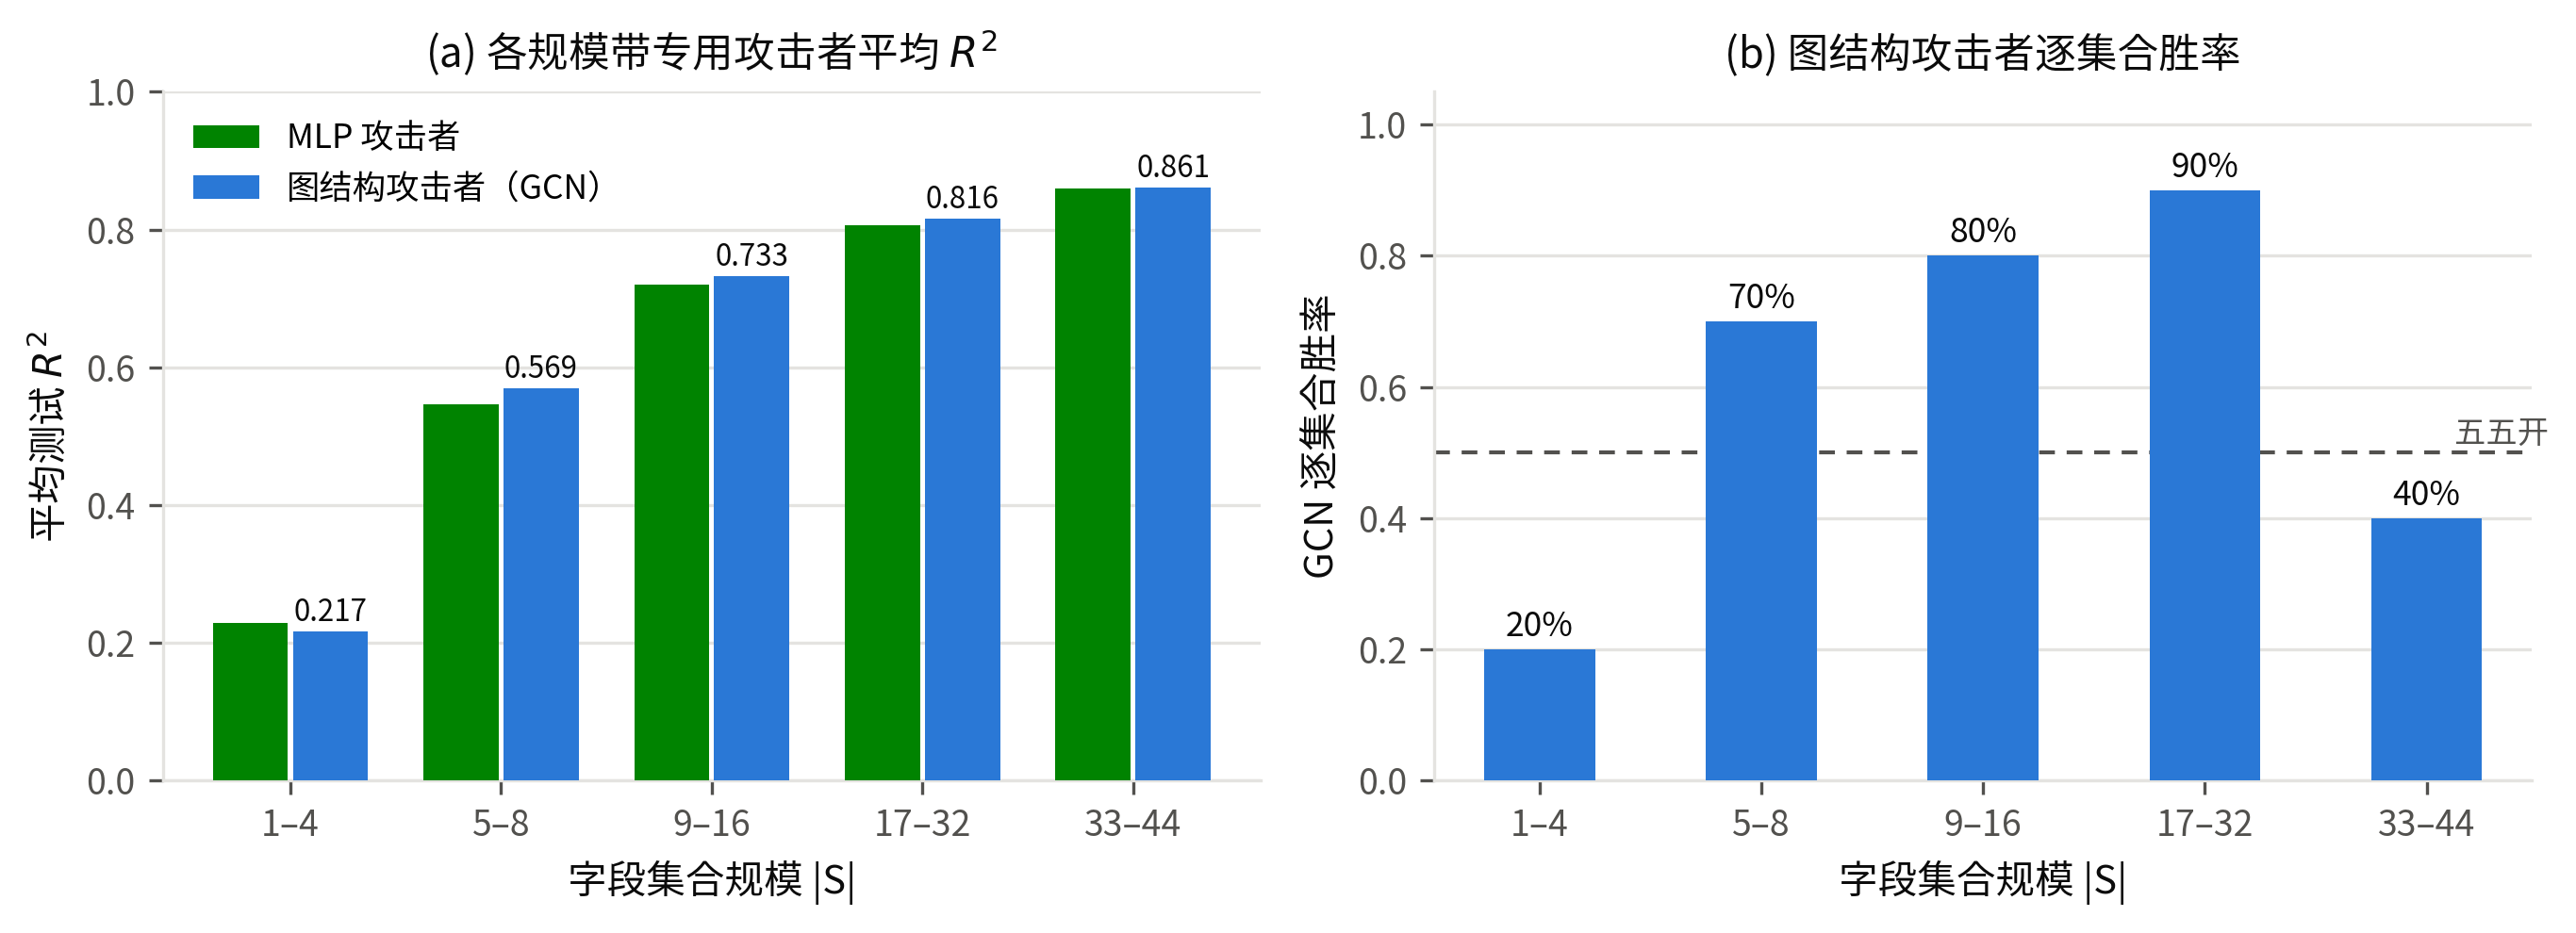
\includegraphics[width=0.98\linewidth]{attacker_compare_zh.png}}
{\heiti 图 1\quad 图结构与 MLP 专用推断模型按集合规模的对比：(a) 平均测试 $R^2$；(b) GCN 逐集合胜率}
\label{fig:attacker}
\end{figure}

\begin{table}[htbp]
\centering {\heiti 表 1\quad 专用推断模型结构对比（重训，按集合类别）}
\vspace {1mm}
\begin{center}
\zihao{5-}
\begin{tabular}{lccccc}
\toprule
集合类别 & 集合数 & MLP 平均 $R^2$ & GCN 平均 $R^2$ & 差值 & GCN 胜率 \\
\midrule
随机集合 1--4 字段   & 10 & 0.228 & 0.217 & $-0.011$ & 20\% \\
随机集合 5--8 字段   & 10 & 0.546 & 0.569 & $+0.023$ & 70\% \\
随机集合 9--16 字段  & 10 & 0.720 & 0.733 & $+0.013$ & 80\% \\
随机集合 17--32 字段 & 10 & 0.807 & 0.816 & $+0.010$ & 90\% \\
随机集合 33--44 字段 & 10 & 0.860 & 0.861 & $+0.001$ & 40\% \\
随机集合合计         & 50 & 0.632 & 0.639 & $+0.007$ & 60\% \\
字段对（审计样本）   & 9  & 0.220 & 0.182 & $-0.038$ & 11\% \\
三元组（审计样本）   & 9  & 0.417 & 0.388 & $-0.029$ & 0\%  \\
\bottomrule
\end{tabular}
\label{tab:attacker}
\end{center}
\end{table}

三点观察：(1) 在 5 字段及以上的随机集合上，图结构攻击者的平均 $R^2$ 全面高于 MLP，其中 5--8 字段段提升 0.023（超过 GCN 显著标尺 0.02），且逐集合胜率随规模从 20\%单调上升至 90\%——集合越大，相关图提供的结构先验越能约束假设空间，图结构的优势越稳定；33--44 字段段两者同时逼近信息上限（$R^2\approx0.86$），差异自然消失。(2) 在极小集合（字段对、三元组审计样本）上图结构无优势，此时图中大量无关节点的消息构成噪声，全连接的 MLP 反而更直接。(3) 两种结构存在互补性：对每个机密字段取两结构较优者，可在单结构基础上再获得 0.005--0.017 的包络增益，故本文以 best-of-struct 作为攻击上限口径。

\subsection{子集条件图 oracle 的保真度}

图 oracle 对重训真值的逼近质量如图 2 与表 2 所示。不微调（$K{=}0$）时，宽尺寸集合的逐机密字段 MAE 为 0.136，集合排序 Spearman 相关已达 0.975——摊销估计的排序信息足以支撑筛选；经 $K{=}200$ 步微调（每集合约 3.1 秒）后，MAE 降至 0.078，字段对与三元组分别降至 0.035 与 0.044，三元组排序相关由 0.846 升至 0.973。以一次约 3 秒的微调前向替代一次完整重训，将任意集合的敏感度评估成本压缩了两个数量级以上。

\begin{figure}[htbp]
\centering
\centerline{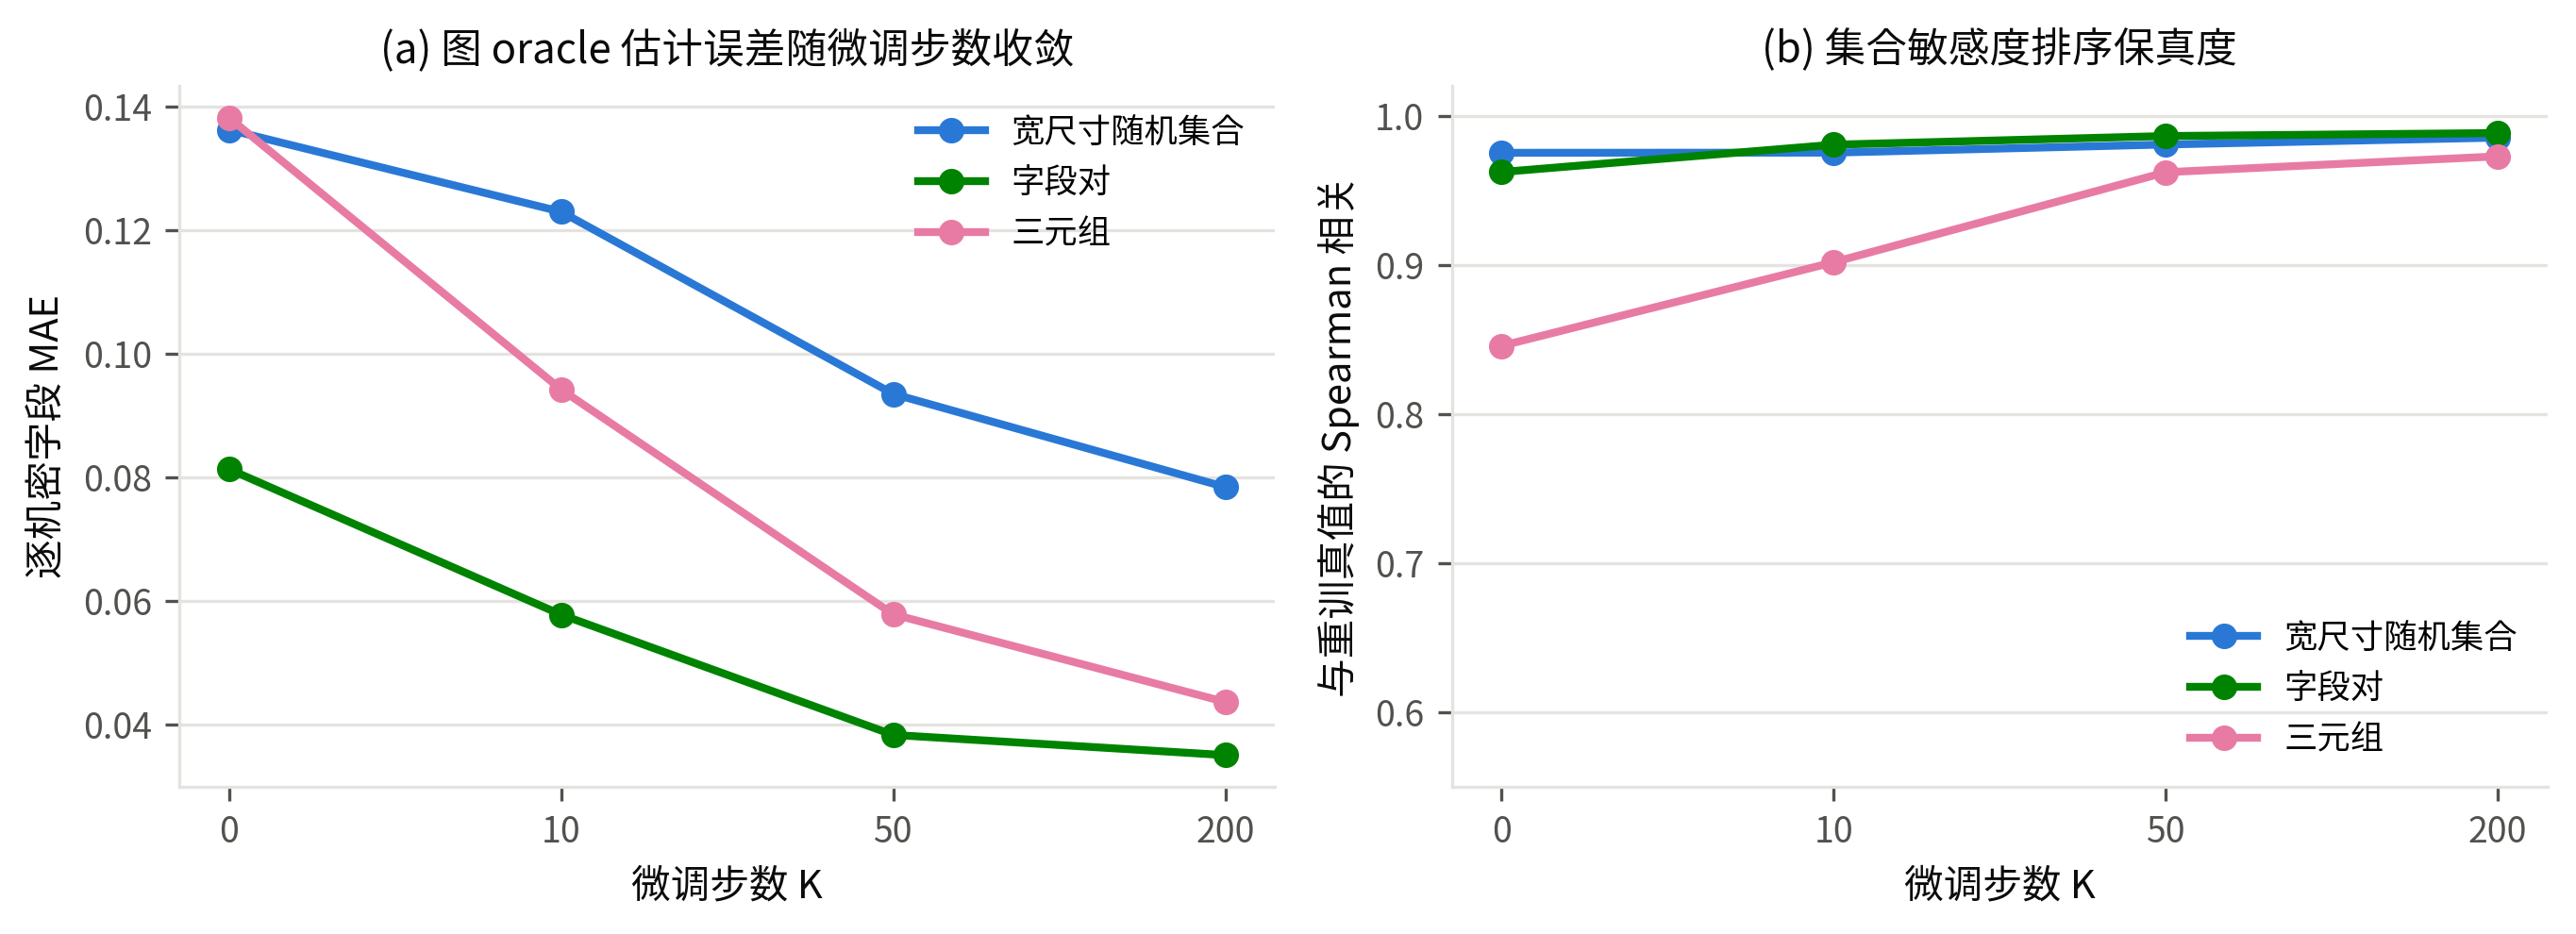
\includegraphics[width=0.98\linewidth]{oracle_fidelity_zh.png}}
{\heiti 图 2\quad 子集条件图 oracle 对重训真值的保真度随微调步数 $K$ 的变化：(a) 逐机密字段 MAE；(b) 集合排序 Spearman 相关}
\label{fig:oracle}
\end{figure}

\begin{table}[htbp]
\centering {\heiti 表 2\quad 图 oracle 保真度（相对全体 MLP 重训真值）}
\vspace {1mm}
\begin{center}
\zihao{5-}
\begin{tabular}{lcccc}
\toprule
集合类别 & MAE ($K{=}0$) & MAE ($K{=}200$) & Spearman ($K{=}0$) & Spearman ($K{=}200$) \\
\midrule
宽尺寸随机集合 & 0.136 & 0.078 & 0.975 & 0.985 \\
字段对         & 0.081 & 0.035 & 0.962 & 0.988 \\
三元组         & 0.138 & 0.044 & 0.846 & 0.973 \\
\bottomrule
\end{tabular}
\label{tab:oracle}
\end{center}
\end{table}

\subsection{二阶协同图与测量口径之争}

对全部 946 个字段对逐一重训，得到二阶协同图的重训真值（图 3）。最强协同均具备清晰物理机制：各类燃料的“出力 MW + 燃料占比”对合体后可精确推断总发电量（总发电 $=$ 出力 $\div$ 占比），如表 3 所示——风电对协同增量达 0.765，太阳能出力单独几乎无泄露（$R^2=0.006$）却参与 0.596 的协同。这类“单看安全、合体泄露”的物理级实证，直接否定了单字段敏感度评分的充分性。

\begin{figure}[htbp]
\centering
\centerline{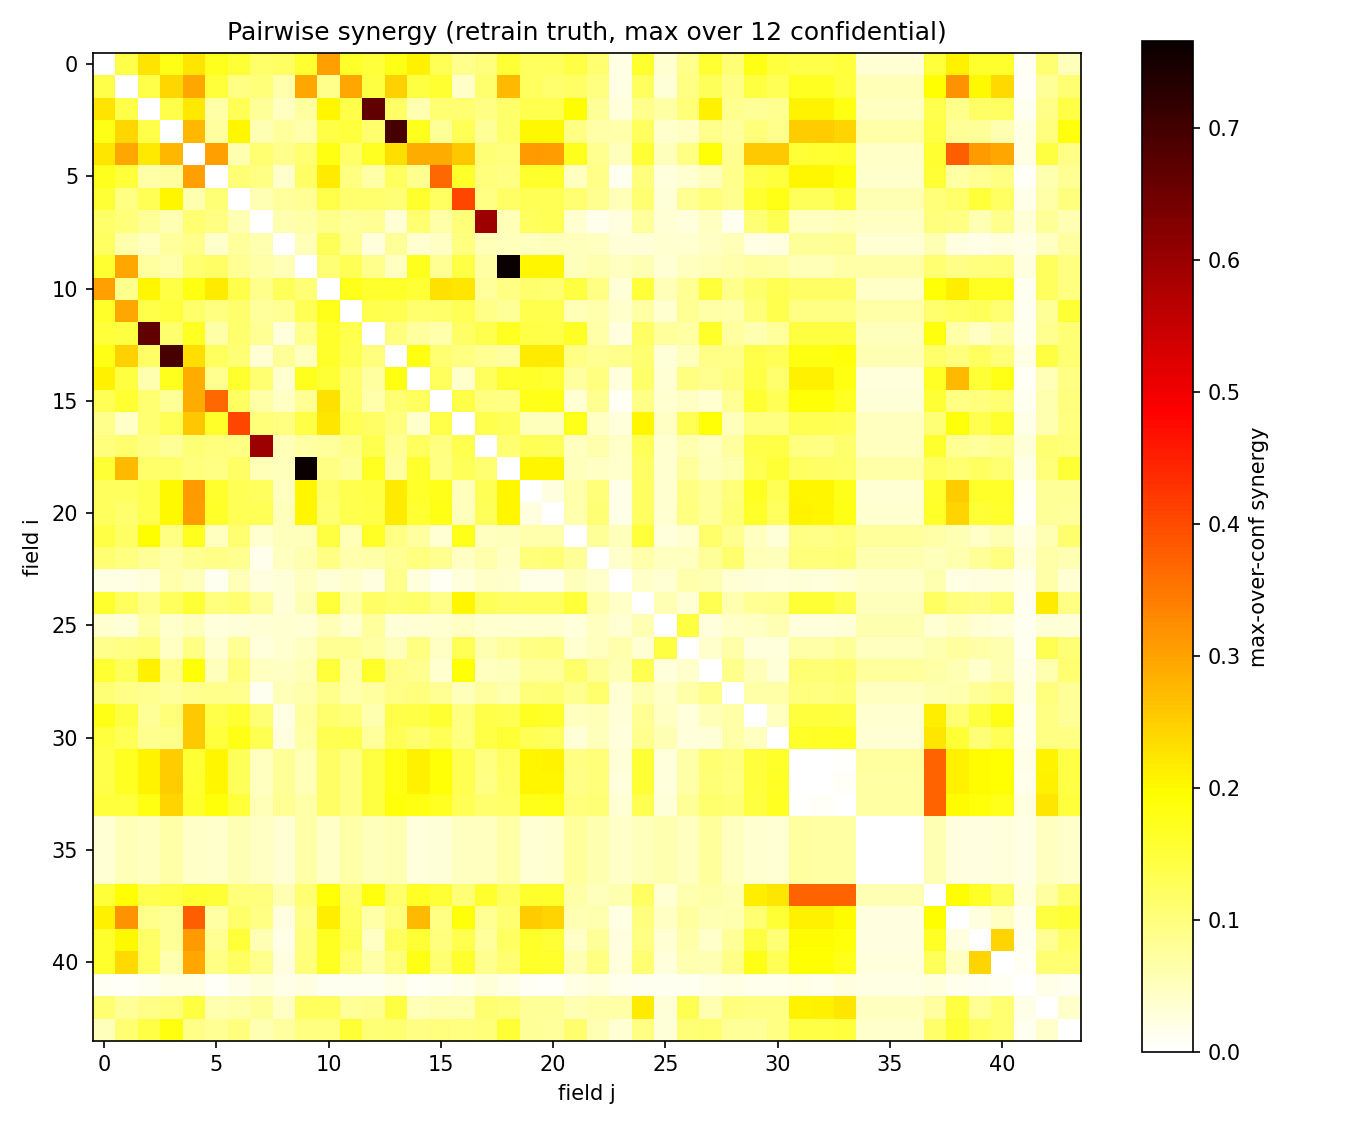
\includegraphics[width=0.72\linewidth]{synergy2_heatmap.png}}
{\heiti 图 3\quad 二阶协同图的邻接矩阵热力图（重训真值，对 12 个机密字段取最大值）。显著协同（深色）集中于少数字段对，呈稀疏结构}
\label{fig:heatmap}
\end{figure}

\begin{table}[htbp]
\centering {\heiti 表 3\quad 最强二阶协同对（重训真值）}
\vspace {1mm}
\begin{center}
\zihao{5-}
\begin{tabular}{llcccc}
\toprule
字段对 & 机密目标 & $v_c(i)$ & $v_c(j)$ & $v_c(\{i,j\})$ & $\mathrm{syn}_2$ \\
\midrule
风电 MW + 风电占比     & 总发电量 & 0.064 & 0.162 & 0.928 & 0.765 \\
多燃料 MW + 多燃料占比 & 总发电量 & 0.201 & 0.078 & 0.897 & 0.696 \\
水电 MW + 水电占比     & 总发电量 & 0.292 & 0.135 & 0.957 & 0.665 \\
太阳能 MW + 太阳能占比 & 总发电量 & 0.006 & 0.099 & 0.695 & 0.596 \\
\bottomrule
\end{tabular}
\label{tab:syn2}
\end{center}
\end{table}

以同一批字段对对比置零口径：置零协同与重训真值的 Spearman 相关仅 0.351，协同均值 0.012 对重训真值 0.041，系统性低估 3.4 倍。置零保持全字段模型参数不变，无法表达“攻击者针对可见集合重新优化”的最优响应语义，因而既低估绝对量、又排不对顺序。忠实的集合敏感度评估必须以重训为真值，廉价口径只能担任筛选角色。

\subsection{三阶协同：全扫描与重训认证}

以 $K{=}200$ 微调 oracle 全扫描 13244 个三元组并按式 (\ref{eq:syn3}) 排序，对 top-200 候选与 200 个随机对照三元组重训认证，结果如图 4 所示。

\begin{figure}[htbp]
\centering
\centerline{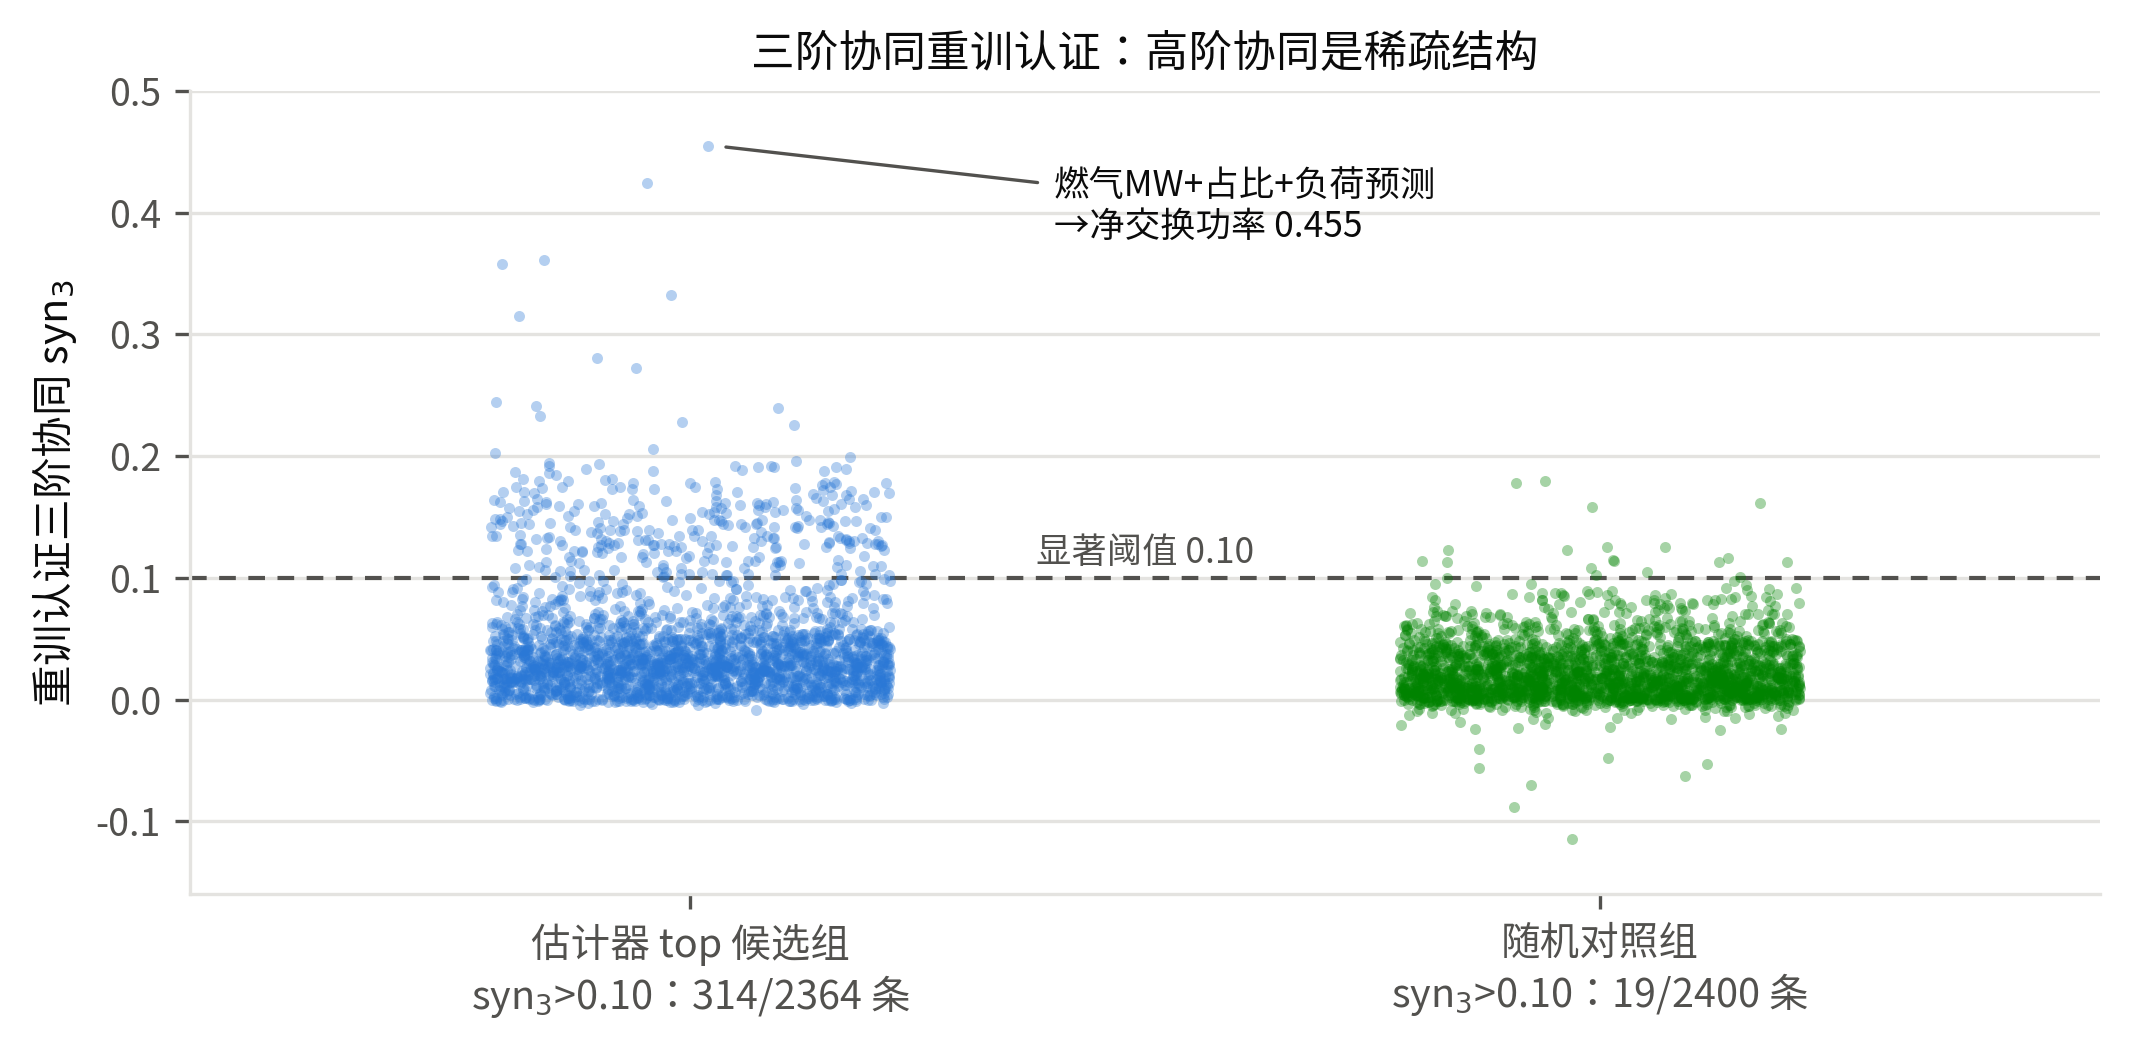
\includegraphics[width=0.85\linewidth]{triple_certify_zh.png}}
{\heiti 图 4\quad 三阶协同重训认证。top 候选组 2364 条认证记录中 314 条超过显著阈值 0.10，随机对照组 2400 条中仅 19 条（中位数 0.018，处于噪声底），高阶协同是稀疏结构}
\label{fig:triple}
\end{figure}

主要结论：(1) \textbf{真不可约三阶协同存在且物理可解释}。最强者为“燃气出力 + 燃气占比 + 负荷预测 $\to$ 净交换功率”，认证值 0.455，其最优二元子集仅 0.24--0.28：净交换在物理上等于发电减负荷，推断发电需要“出力 + 占比”两字段、推断负荷需要“负荷预测”一字段，三者缺一不可；燃煤、核电、水电、风电的同构三元组认证值为 0.24--0.42。(2) \textbf{扫描—认证协议可靠}。估计与认证排序 Spearman 相关 0.795，且估计系统性保守（最强项估计 0.421 对认证 0.455），保证 top 筛选不漏强项。(3) \textbf{高阶协同稀疏}。随机对照组几乎不含显著三阶协同（19/2400，中位数 0.018 处于噪声底），显著协同集中于少数具有物理合成关系的三元组。该稀疏性意味着协同超图 $H_{\mathrm{syn}}$ 的显著超边极少，也为更高阶搜索提供了剪枝依据——高阶候选可以只在已认证的低阶强协同的超集中生成，类似频繁项集挖掘的先验式剪枝。

\section{\heiti 讨论}

\textbf{图结构的适用边界}。实验将图结构的收益定位于两处：其一是中大规模集合的专用推断（5--32 字段段平均 $R^2$ 与胜率的系统性优势），其二是结构互补带来的攻击上限包络增益。同时也应指出，在摊销 oracle 这一角色上，同等优化步数下更简单的 MLP 估计器在绝对误差上仍具竞争力，图结构 oracle 的相对优势主要体现在集合排序保真度已足够支撑扫描协议（Spearman 0.97 以上）而非逐点精度。这与关系归纳偏置的一般规律一致\upcite{battaglia2018relational,grinsztajn2022tabular}：图先验在依赖结构与图拓扑对齐时获益最大，而对任意掩码模式的摊销回归更接近无结构的表格学习。

\textbf{可迁移性}。图结构模型的参数由共享的消息函数与注意力函数构成，与字段数量、字段身份解耦；节点仅需去身份化的统计特征即可表示。这意味着在字段集不同的另一电网系统上，图攻击者与图 oracle 原则上可以直接迁移或少样本适配，而 MLP 的输入维度与字段顺序绑定、结构上无法跨系统复用。跨系统迁移（如在 IEEE 标准算例系统上与 IGNN 正面对比）是本框架最自然的下一步，本文暂以分析性论证给出，实验验证留作未来工作。

\textbf{可扩展性}。三阶实验揭示的协同稀疏性提示 $v_c(S)$ 可能具有低阶稀疏结构（布尔函数意义上的低度数近似\upcite{odonnell2014boolean}）：若 $v_c$ 能被单字段、显著字段对与显著三元组的低阶项良好重构，则任意集合的敏感度评估从 $2^n$ 塌缩为 $O(n^2)$--$O(n^3)$ 个系数的查表与组合，配合先验式剪枝可将框架推广到字段数更多的系统。

\textbf{局限}。(1) 字段对与三元组上的 GCN 结果来自各 9 个分层审计样本，不应外推为穷举结论；(2) 三阶 top 候选来自估计器扫描，存在选择偏差，故结论同时依赖随机对照组；(3) 协同显著阈值 0.10 是基于噪声底的经验选择。

\section{\heiti 结论}

本文将电网数据推断泄露的敏感度评估从单字段分数升维为任意字段集合上的集合函数，并给出以图结构为骨架的完整评估框架：字段相关图上的专用推断模型刻画攻击上限（中大规模集合上系统性优于 MLP，胜率随规模升至 90\%）；子集条件图 oracle 配合秒级微调将单集合评估成本压缩两个数量级（MAE 0.078，排序相关 0.97 以上）；扫描—认证协议在 13244 个三元组的组合空间中可靠定位真不可约三阶协同（最强 0.455，估计—认证排序相关 0.795 且保守）。实验同时证明高阶协同泄露是稀疏且物理可解释的结构，而置零式评估口径会低估协同 3.4 倍——集合语义、重训真值与图结构组织三者共同构成忠实敏感度评估的方法学基础。未来工作将沿低阶稀疏重构与跨系统迁移两个方向推进。

%%%%%%%%%%%%%%%%%%%%%%%%%%%%%%%%%
\vspace {10mm}
\centerline
{\zihao{5}\textsf{参~考~文~献}}
\zihao{5-} \addtolength{\itemsep}{-1em}
\vspace {1.5mm}
\bibliographystyle{gbt7714-numerical}
\bibliography{ref.bib}

\end{document}
